\documentclass[12pt]{article}
\usepackage{multicol}
\usepackage[shortlabels]{enumitem}
\usepackage{tikz}
\usepackage{tikz-qtree}
\usepackage{tipa}
\begin{document}
\title{Linguistics 20, Homework 5}
\date{May 6th, 2019}
\author{Michael Wu\\UID: 404751542\\TA: Eleanor Glewwe\\Discussion 1F Friday 9:00-9:50 AM}
\maketitle

\section*{Chapter 4, Problem 9}

\paragraph{i)}

\tikzset{level distance = 1.7cm}
\begin{multicols}{3}
    \begin{enumerate}
        \item[a)] desks
        \begin{center}
            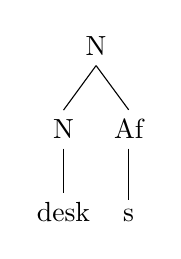
\begin{tikzpicture}
                \Tree [.N [.N desk ] [.Af s ] ]
            \end{tikzpicture}
        \end{center}
        \item[c)] insincere
        \begin{center}
            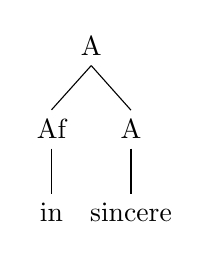
\begin{tikzpicture}
                \Tree [.A [.Af in ] [.A sincere ] ]
            \end{tikzpicture}
        \end{center}
        \item[e)] triumphed
        \begin{center}
            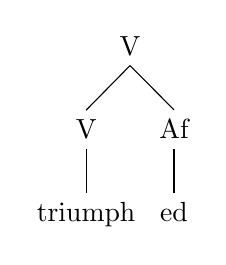
\begin{tikzpicture}
                \Tree [.V [.V triumph ] [.Af ed ] ]
            \end{tikzpicture}
        \end{center}
        \item[h)] payment
        \begin{center}
            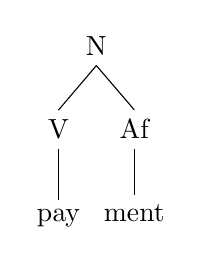
\begin{tikzpicture}
                \Tree [.N [.V pay ] [.Af ment ] ]
            \end{tikzpicture}
        \end{center}
        \item[k)] redistribute
        \begin{center}
            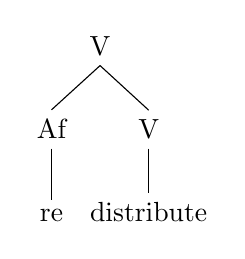
\begin{tikzpicture}
                \Tree [.V [.Af re ] [.V distribute ] ]
            \end{tikzpicture}
        \end{center}
        \item[m)] optionality
        \begin{center}
            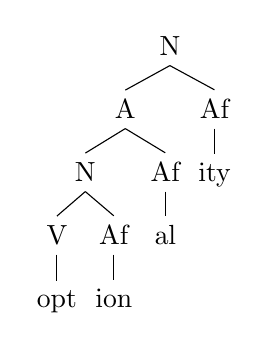
\begin{tikzpicture}[sibling distance = 0cm, level distance = 0.8cm]
                \Tree [.N [.A [.N [.V opt ] [.Af ion ] ] [.Af al ] ] [.Af ity ] ]
            \end{tikzpicture}
        \end{center}
    \end{enumerate}
\end{multicols}

\paragraph{ii)}

The base for the affix -ion is opt. The base for the suffix -ity is optional. The base opt is the root of
the entire word.

\section*{Chapter 4, Problem 10}

\paragraph{i)}

The affix -em- converts nouns to verbs.

\paragraph{ii)}

It is an infix.

\section*{Chapter 4, Problem 12}

\paragraph{i)}

The suffix -er in these words mean ``someone who is from here''.

\paragraph{ii)}

It is different because this -er has a noun as a base, whereas the -er in
skater has a verb as a base and means ``someone who does this''.

\paragraph{iii)}

The suffix -er when used on a place should not come after liquids or vowels.

\paragraph{iv)}

The previous constraint does not apply to the -er that is applied to verbs.
For example the words doer, stutterer, and caller are all valid words.

\section*{Chapter 4, Problem 13}

\tikzset{level distance = 1cm, sibling distance = 0cm, every picture/.style={scale = 0.9}}
\begin{multicols}{4}
    \begin{enumerate}
        \item[a)] football
        \begin{center}
            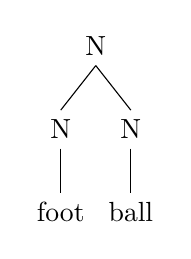
\begin{tikzpicture}
                \Tree [.N [.N foot ] [.N ball ] ]
            \end{tikzpicture}
        \end{center}
        \item[e)] fast food
        \begin{center}
            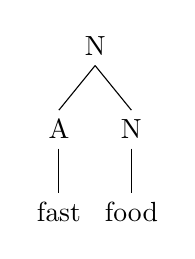
\begin{tikzpicture}
                \Tree [.N [.A fast ] [.N food ] ]
            \end{tikzpicture}
        \end{center}
        \item[m)] city center
        \begin{center}
            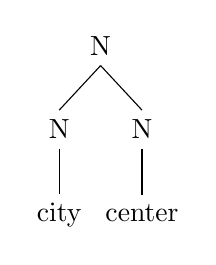
\begin{tikzpicture}
                \Tree [.N [.N city ] [.N center ] ]
            \end{tikzpicture}
        \end{center}
        \item[v)] space ship
        \begin{center}
            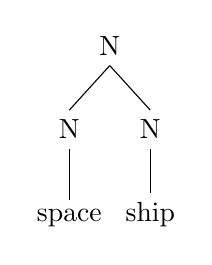
\begin{tikzpicture}
                \Tree [.N [.N space ] [.N ship ] ]
            \end{tikzpicture}
        \end{center}
    \end{enumerate}
\end{multicols}

\section*{Chapter 4, Problem 18}

\paragraph{i)}

In the first column, inflection is expressed by making an internal change to the vowel sound. In the second column,
inflection is expressed through suppletion and the entire word is changed. In the third column, the suffix -ed is added
to express inflection.

\section*{Study Guide Chapter 4, Problem 6}

\paragraph{a)}

\begin{multicols}{2}
    \begin{enumerate}
        \item I, -it
        \item we, -na
        \item you (M SG), -it
        \item you (F SG), -ti
        \item you (PL), -tu
        \item he, implicit with no extra morpheme
        \item she, -at
        \item they, -aw
    \end{enumerate}
\end{multicols}

\paragraph{b)}

The last vowel of the word is removed.

\paragraph{c)}

[t\textsuperscript{\textrevglotstop}ubaxit]

\end{document}